\documentclass[twoside]{book}

% Packages required by doxygen
\usepackage{fixltx2e}
\usepackage{calc}
\usepackage{doxygen}
\usepackage[export]{adjustbox} % also loads graphicx
\usepackage{graphicx}
\usepackage[utf8]{inputenc}
\usepackage{makeidx}
\usepackage{multicol}
\usepackage{multirow}
\PassOptionsToPackage{warn}{textcomp}
\usepackage{textcomp}
\usepackage[nointegrals]{wasysym}
\usepackage[table]{xcolor}

% Font selection
\usepackage[T1]{fontenc}
\usepackage[scaled=.90]{helvet}
\usepackage{courier}
\usepackage{amssymb}
\usepackage{sectsty}
\renewcommand{\familydefault}{\sfdefault}
\allsectionsfont{%
  \fontseries{bc}\selectfont%
  \color{darkgray}%
}
\renewcommand{\DoxyLabelFont}{%
  \fontseries{bc}\selectfont%
  \color{darkgray}%
}
\newcommand{\+}{\discretionary{\mbox{\scriptsize$\hookleftarrow$}}{}{}}

% Page & text layout
\usepackage{geometry}
\geometry{%
  a4paper,%
  top=2.5cm,%
  bottom=2.5cm,%
  left=2.5cm,%
  right=2.5cm%
}
\tolerance=750
\hfuzz=15pt
\hbadness=750
\setlength{\emergencystretch}{15pt}
\setlength{\parindent}{0cm}
\setlength{\parskip}{3ex plus 2ex minus 2ex}
\makeatletter
\renewcommand{\paragraph}{%
  \@startsection{paragraph}{4}{0ex}{-1.0ex}{1.0ex}{%
    \normalfont\normalsize\bfseries\SS@parafont%
  }%
}
\renewcommand{\subparagraph}{%
  \@startsection{subparagraph}{5}{0ex}{-1.0ex}{1.0ex}{%
    \normalfont\normalsize\bfseries\SS@subparafont%
  }%
}
\makeatother

% Headers & footers
\usepackage{fancyhdr}
\pagestyle{fancyplain}
\fancyhead[LE]{\fancyplain{}{\bfseries\thepage}}
\fancyhead[CE]{\fancyplain{}{}}
\fancyhead[RE]{\fancyplain{}{\bfseries\leftmark}}
\fancyhead[LO]{\fancyplain{}{\bfseries\rightmark}}
\fancyhead[CO]{\fancyplain{}{}}
\fancyhead[RO]{\fancyplain{}{\bfseries\thepage}}
\fancyfoot[LE]{\fancyplain{}{}}
\fancyfoot[CE]{\fancyplain{}{}}
\fancyfoot[RE]{\fancyplain{}{\bfseries\scriptsize Generated by Doxygen }}
\fancyfoot[LO]{\fancyplain{}{\bfseries\scriptsize Generated by Doxygen }}
\fancyfoot[CO]{\fancyplain{}{}}
\fancyfoot[RO]{\fancyplain{}{}}
\renewcommand{\footrulewidth}{0.4pt}
\renewcommand{\chaptermark}[1]{%
  \markboth{#1}{}%
}
\renewcommand{\sectionmark}[1]{%
  \markright{\thesection\ #1}%
}

% Indices & bibliography
\usepackage{natbib}
\usepackage[titles]{tocloft}
\setcounter{tocdepth}{3}
\setcounter{secnumdepth}{5}
\makeindex

% Hyperlinks (required, but should be loaded last)
\usepackage{ifpdf}
\ifpdf
  \usepackage[pdftex,pagebackref=true]{hyperref}
\else
  \usepackage[ps2pdf,pagebackref=true]{hyperref}
\fi
\hypersetup{%
  colorlinks=true,%
  linkcolor=blue,%
  citecolor=blue,%
  unicode%
}

% Custom commands
\newcommand{\clearemptydoublepage}{%
  \newpage{\pagestyle{empty}\cleardoublepage}%
}

\usepackage{caption}
\captionsetup{labelsep=space,justification=centering,font={bf},singlelinecheck=off,skip=4pt,position=top}

%===== C O N T E N T S =====

\begin{document}

% Titlepage & ToC
\hypersetup{pageanchor=false,
             bookmarksnumbered=true,
             pdfencoding=unicode
            }
\pagenumbering{alph}
\begin{titlepage}
\vspace*{7cm}
\begin{center}%
{\Large Boussinesq }\\
\vspace*{1cm}
{\large Generated by Doxygen 1.8.12}\\
\end{center}
\end{titlepage}
\clearemptydoublepage
\pagenumbering{roman}
\tableofcontents
\clearemptydoublepage
\pagenumbering{arabic}
\hypersetup{pageanchor=true}

%--- Begin generated contents ---
\chapter{Hierarchical Index}
\section{Class Hierarchy}
This inheritance list is sorted roughly, but not completely, alphabetically\+:\begin{DoxyCompactList}
\item object\begin{DoxyCompactList}
\item \contentsline{section}{Boussinesq\+Simulation.\+Boussinesq\+Simulation}{\pageref{class_boussinesq_simulation_1_1_boussinesq_simulation}}{}
\item \contentsline{section}{Hs1\+D.\+Hs1D}{\pageref{class_hs1_d_1_1_hs1_d}}{}
\item \contentsline{section}{Simulation\+Results.\+Simulation\+Results}{\pageref{class_simulation_results_1_1_simulation_results}}{}
\item \contentsline{section}{Source.\+Source}{\pageref{class_source_1_1_source}}{}
\item \contentsline{section}{Space\+Discretization.\+Space\+Discretization}{\pageref{class_space_discretization_1_1_space_discretization}}{}
\end{DoxyCompactList}
\end{DoxyCompactList}

\chapter{Class Index}
\section{Class List}
Here are the classes, structs, unions and interfaces with brief descriptions\+:\begin{DoxyCompactList}
\item\contentsline{section}{\hyperlink{class_boussinesq_simulation_1_1_boussinesq_simulation}{Boussinesq\+Simulation.\+Boussinesq\+Simulation} }{\pageref{class_boussinesq_simulation_1_1_boussinesq_simulation}}{}
\item\contentsline{section}{\hyperlink{class_hs1_d_1_1_hs1_d}{Hs1\+D.\+Hs1D} }{\pageref{class_hs1_d_1_1_hs1_d}}{}
\item\contentsline{section}{\hyperlink{class_simulation_results_1_1_simulation_results}{Simulation\+Results.\+Simulation\+Results} }{\pageref{class_simulation_results_1_1_simulation_results}}{}
\item\contentsline{section}{\hyperlink{class_source_1_1_source}{Source.\+Source} }{\pageref{class_source_1_1_source}}{}
\item\contentsline{section}{\hyperlink{class_space_discretization_1_1_space_discretization}{Space\+Discretization.\+Space\+Discretization} }{\pageref{class_space_discretization_1_1_space_discretization}}{}
\end{DoxyCompactList}

\chapter{Class Documentation}
\hypertarget{class_boussinesq_simulation_1_1_boussinesq_simulation}{}\section{Boussinesq\+Simulation.\+Boussinesq\+Simulation Class Reference}
\label{class_boussinesq_simulation_1_1_boussinesq_simulation}\index{Boussinesq\+Simulation.\+Boussinesq\+Simulation@{Boussinesq\+Simulation.\+Boussinesq\+Simulation}}
Inheritance diagram for Boussinesq\+Simulation.\+Boussinesq\+Simulation\+:\begin{figure}[H]
\begin{center}
\leavevmode
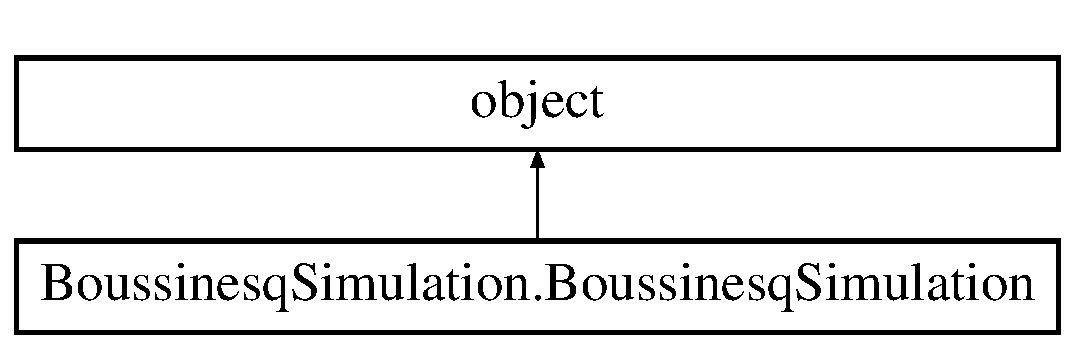
\includegraphics[height=2.000000cm]{class_boussinesq_simulation_1_1_boussinesq_simulation}
\end{center}
\end{figure}


The documentation for this class was generated from the following file\+:\begin{DoxyCompactItemize}
\item 
process/simulation/Boussinesq\+Simulation.\+py\end{DoxyCompactItemize}

\hypertarget{class_hs1_d_1_1_hs1_d}{}\section{Hs1\+D.\+Hs1D Class Reference}
\label{class_hs1_d_1_1_hs1_d}\index{Hs1\+D.\+Hs1D@{Hs1\+D.\+Hs1D}}
Inheritance diagram for Hs1\+D.\+Hs1D\+:\begin{figure}[H]
\begin{center}
\leavevmode
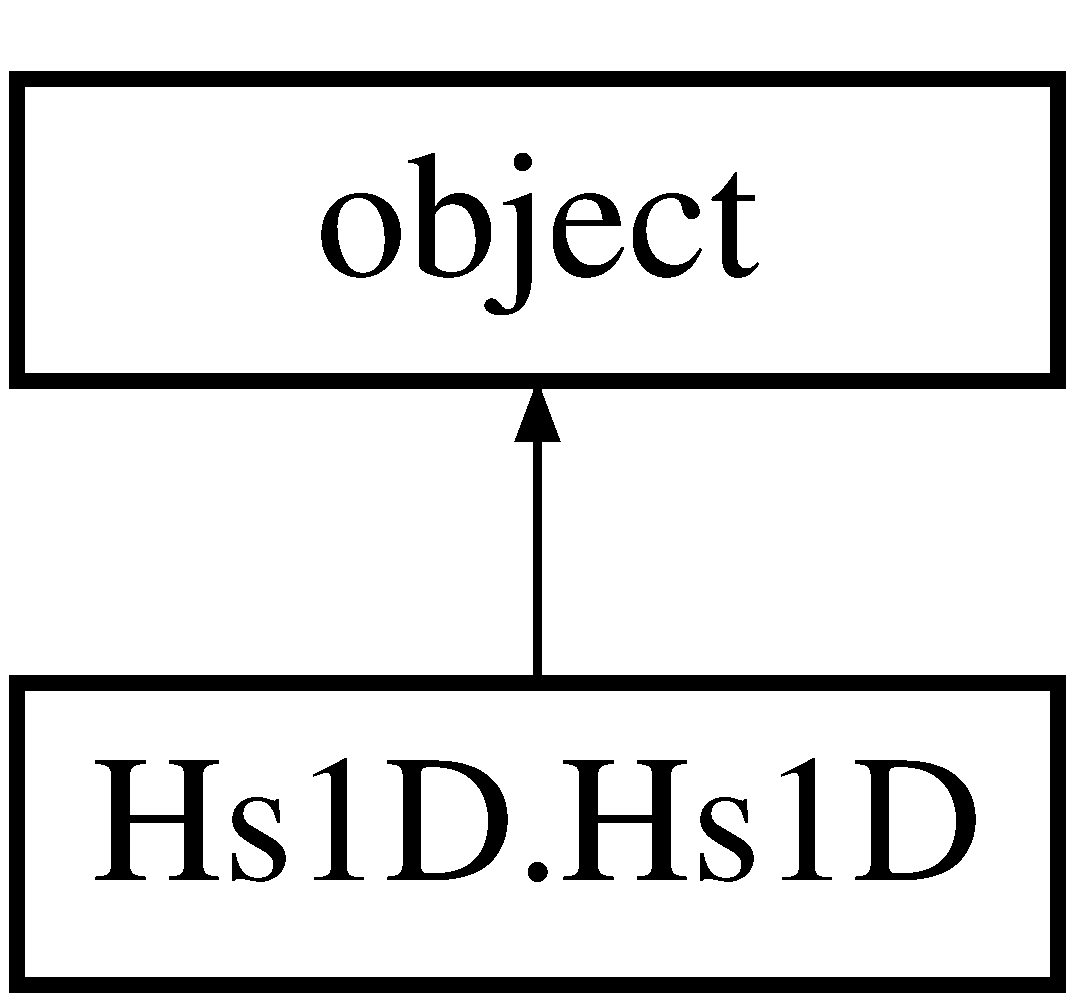
\includegraphics[height=2.000000cm]{class_hs1_d_1_1_hs1_d}
\end{center}
\end{figure}
\subsection*{Public Member Functions}
\begin{DoxyCompactItemize}
\item 
\hypertarget{class_hs1_d_1_1_hs1_d_a941546c82bf143abe81b50e5aa776974}{}\label{class_hs1_d_1_1_hs1_d_a941546c82bf143abe81b50e5aa776974} 
def {\bfseries \+\_\+\+\_\+init\+\_\+\+\_\+} (self, nx, angle, w, soil\+\_\+depth, k, f, z\+\_\+custom, x)
\item 
\hypertarget{class_hs1_d_1_1_hs1_d_a609192fa9038f7ab060dab430637236f}{}\label{class_hs1_d_1_1_hs1_d_a609192fa9038f7ab060dab430637236f} 
def {\bfseries get\+\_\+w\+\_\+edges} (self)
\item 
\hypertarget{class_hs1_d_1_1_hs1_d_a7205363d9052b79d7634262ea5ffc6a8}{}\label{class_hs1_d_1_1_hs1_d_a7205363d9052b79d7634262ea5ffc6a8} 
def {\bfseries get\+\_\+soil\+\_\+depth\+\_\+edges} (self)
\item 
\hypertarget{class_hs1_d_1_1_hs1_d_a7690c0b1b76d9bd363fb1e02f581f4e8}{}\label{class_hs1_d_1_1_hs1_d_a7690c0b1b76d9bd363fb1e02f581f4e8} 
def {\bfseries get\+\_\+angle\+\_\+edges} (self)
\item 
\hypertarget{class_hs1_d_1_1_hs1_d_a1460c5bbb135a1b55529600e1b1f5bbd}{}\label{class_hs1_d_1_1_hs1_d_a1460c5bbb135a1b55529600e1b1f5bbd} 
def {\bfseries get\+\_\+k} (self)
\item 
\hypertarget{class_hs1_d_1_1_hs1_d_a41d0dc149f791ed7a1238f0757fe5cdd}{}\label{class_hs1_d_1_1_hs1_d_a41d0dc149f791ed7a1238f0757fe5cdd} 
def {\bfseries get\+\_\+f} (self)
\end{DoxyCompactItemize}
\subsection*{Public Attributes}
\begin{DoxyCompactItemize}
\item 
\hypertarget{class_hs1_d_1_1_hs1_d_afa750ce5872c1ac79c30fbacd814d9dc}{}\label{class_hs1_d_1_1_hs1_d_afa750ce5872c1ac79c30fbacd814d9dc} 
{\bfseries angle\+\_\+edges}
\item 
\hypertarget{class_hs1_d_1_1_hs1_d_a71848087a0eaac7de043027b19f54545}{}\label{class_hs1_d_1_1_hs1_d_a71848087a0eaac7de043027b19f54545} 
{\bfseries w\+\_\+edges}
\item 
\hypertarget{class_hs1_d_1_1_hs1_d_a4d1deaffe02916f21684764b9720d7dd}{}\label{class_hs1_d_1_1_hs1_d_a4d1deaffe02916f21684764b9720d7dd} 
{\bfseries soil\+\_\+depth\+\_\+edges}
\item 
\hypertarget{class_hs1_d_1_1_hs1_d_a4de82095ad48fe85c6c090328f51503d}{}\label{class_hs1_d_1_1_hs1_d_a4de82095ad48fe85c6c090328f51503d} 
{\bfseries k}
\item 
\hypertarget{class_hs1_d_1_1_hs1_d_a02cd319218a500edd69c52c74a6404b7}{}\label{class_hs1_d_1_1_hs1_d_a02cd319218a500edd69c52c74a6404b7} 
{\bfseries f}
\end{DoxyCompactItemize}


\subsection{Detailed Description}
\begin{DoxyVerb}    Class containing the hillslope properties. It's an attribute of
    SpaceDiscretization Class
    #######################################################################
    @☺param
        xmin : minimal coordinate of the hillslope (in meters)
        xmax : maximal coordinate of the hillslope (in meters)
        nx : number of meshes used to describe the hillslope
        angle : slope of the hillslope on each mesh
        w : width of the hillslope on each mesh
        soil_depth : depth of the reservoir on each mesh
        k : hydraulic conductivity on the hillslope (in m/s)
        f : kinematic porosity on the hillslope

    @attributes:
      k : hydraulic conductivity
      f : porosity
      angle_edges : slope on edges
      soil_depth_edges : thickness of the layer on edges
      w_edges : width on edges
    WARNING ! Each property is defined over the edges of the mesh
    #######################################################################
\end{DoxyVerb}
 

The documentation for this class was generated from the following file\+:\begin{DoxyCompactItemize}
\item 
process/simulation/Hs1\+D.\+py\end{DoxyCompactItemize}

\hypertarget{class_simulation_results_1_1_simulation_results}{}\section{Simulation\+Results.\+Simulation\+Results Class Reference}
\label{class_simulation_results_1_1_simulation_results}\index{Simulation\+Results.\+Simulation\+Results@{Simulation\+Results.\+Simulation\+Results}}
Inheritance diagram for Simulation\+Results.\+Simulation\+Results\+:\begin{figure}[H]
\begin{center}
\leavevmode
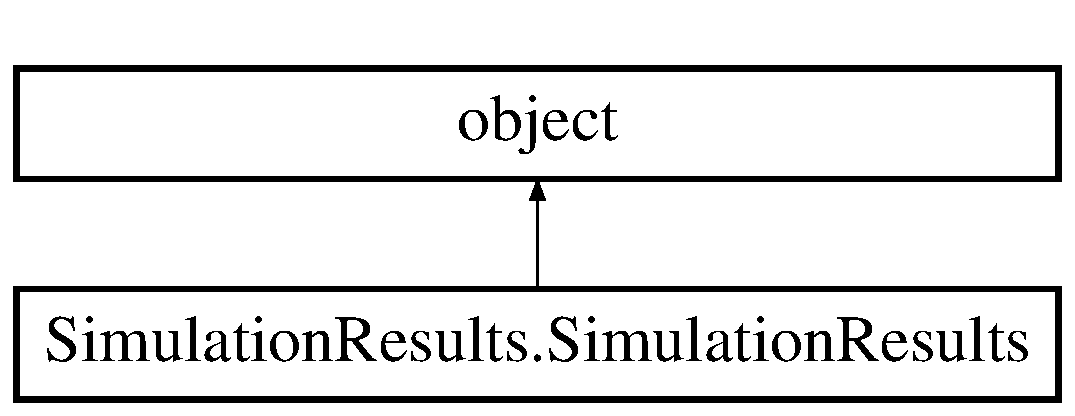
\includegraphics[height=2.000000cm]{class_simulation_results_1_1_simulation_results}
\end{center}
\end{figure}
\subsection*{Public Member Functions}
\begin{DoxyCompactItemize}
\item 
\hypertarget{class_simulation_results_1_1_simulation_results_a3200d3c4ed2fa4acab7420e20109a463}{}\label{class_simulation_results_1_1_simulation_results_a3200d3c4ed2fa4acab7420e20109a463} 
def {\bfseries \+\_\+\+\_\+init\+\_\+\+\_\+} (self, t\+\_\+res, y\+\_\+res, N\+\_\+nodes, N\+\_\+edges, x\+\_\+node, x\+\_\+edges, recharge, dx)
\end{DoxyCompactItemize}
\subsection*{Public Attributes}
\begin{DoxyCompactItemize}
\item 
\hypertarget{class_simulation_results_1_1_simulation_results_abccffd7928439dba5f3f950bf099aef1}{}\label{class_simulation_results_1_1_simulation_results_abccffd7928439dba5f3f950bf099aef1} 
{\bfseries t}
\item 
\hypertarget{class_simulation_results_1_1_simulation_results_acadc2a7467b12f9551c0e918dfe7122f}{}\label{class_simulation_results_1_1_simulation_results_acadc2a7467b12f9551c0e918dfe7122f} 
{\bfseries S}
\item 
\hypertarget{class_simulation_results_1_1_simulation_results_a276ffcb6d07965f631c40a5d43488ecd}{}\label{class_simulation_results_1_1_simulation_results_a276ffcb6d07965f631c40a5d43488ecd} 
{\bfseries Q}
\item 
\hypertarget{class_simulation_results_1_1_simulation_results_aa602d8b25d5c58039c26266e03899e46}{}\label{class_simulation_results_1_1_simulation_results_aa602d8b25d5c58039c26266e03899e46} 
{\bfseries QS}
\item 
\hypertarget{class_simulation_results_1_1_simulation_results_a33b8a52b499f14d9c449238fab6d2ccb}{}\label{class_simulation_results_1_1_simulation_results_a33b8a52b499f14d9c449238fab6d2ccb} 
{\bfseries x\+\_\+node}
\item 
\hypertarget{class_simulation_results_1_1_simulation_results_aa86e9e7f40c34451bad878f359bb4871}{}\label{class_simulation_results_1_1_simulation_results_aa86e9e7f40c34451bad878f359bb4871} 
{\bfseries x\+\_\+edges}
\end{DoxyCompactItemize}


\subsection{Detailed Description}
\begin{DoxyVerb}    Class storing the results of the integration (using IDA solver)

    @param:
      - t_res : times for which the system is solved (s)
      - y_res : the output of the solver for each time (m², m3/s, m²/s)
      - N_nodes : number of cells in the system (-)
      - N_edges : number of cell edges in the system (=N_nodes + 1) (-)
      - x_node : coordinates of cells centers (m)
      - x_edges : coordinates of cells edges (m)
      - recharge : recharge applied to the system (m/s)
      - dx : size of the cells along the hillslope

    @attributes:
      - t : times for which the system is solved (s)
      - S : stock in each cell as a function of time(lines) and x(columns) (m²)
      - Q : flowrate at each cell edge as a function of time(lines) and x(columns) (m3/s)
      - QS : seepage in each cell as a function of time(lines) and x(columns) (m3/s)
      - x_node : coordinates of cells centers (m)
      - x_edges : coordinates of cells edges (m)
\end{DoxyVerb}
 

The documentation for this class was generated from the following file\+:\begin{DoxyCompactItemize}
\item 
process/simulation/Simulation\+Results.\+py\end{DoxyCompactItemize}

\hypertarget{class_source_1_1_source}{}\section{Source.\+Source Class Reference}
\label{class_source_1_1_source}\index{Source.\+Source@{Source.\+Source}}
Inheritance diagram for Source.\+Source\+:\begin{figure}[H]
\begin{center}
\leavevmode
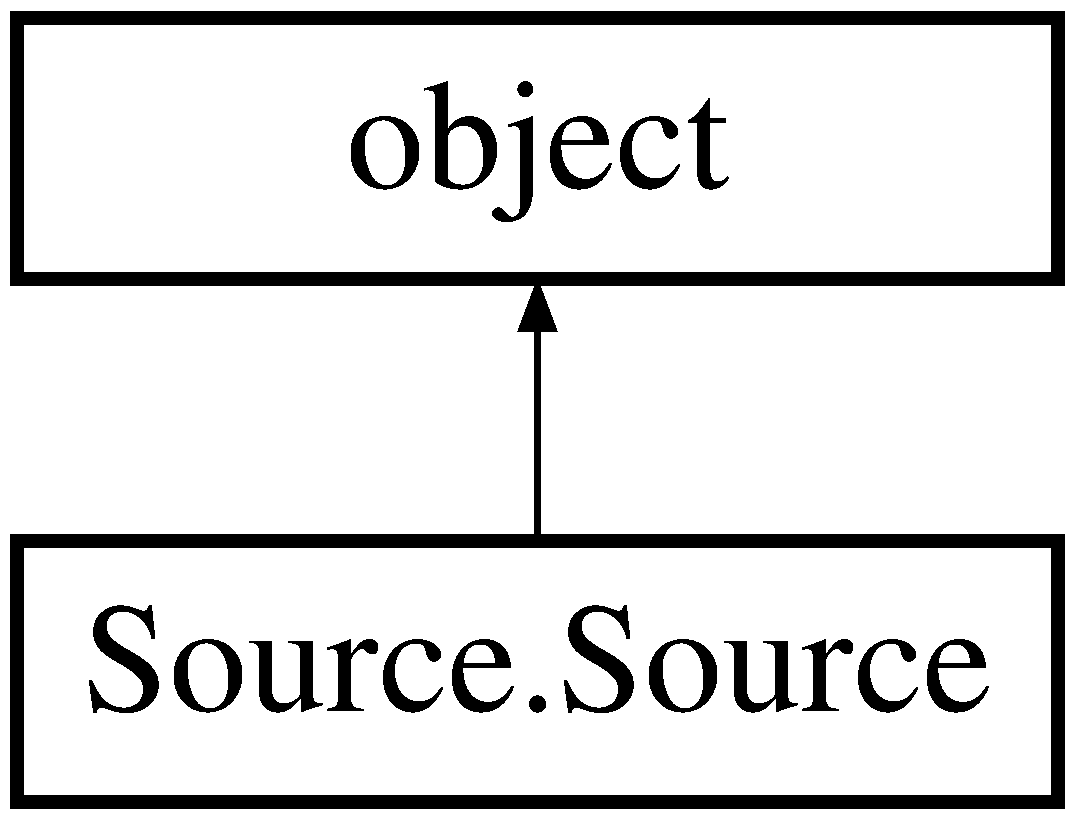
\includegraphics[height=2.000000cm]{class_source_1_1_source}
\end{center}
\end{figure}
\subsection*{Public Member Functions}
\begin{DoxyCompactItemize}
\item 
\hypertarget{class_source_1_1_source_a21a8e2f4c830accec0b97c88c5f9cce7}{}\label{class_source_1_1_source_a21a8e2f4c830accec0b97c88c5f9cce7} 
def {\bfseries \+\_\+\+\_\+init\+\_\+\+\_\+} (self, period, recharge\+\_\+type, recharge\+\_\+rate, tmin, tmax, Nt, unit, time\+\_\+custom)
\item 
\hypertarget{class_source_1_1_source_a4f3c35b4a72dae0b6875e0370baaf15b}{}\label{class_source_1_1_source_a4f3c35b4a72dae0b6875e0370baaf15b} 
def {\bfseries source\+\_\+terms} (self)
\item 
\hypertarget{class_source_1_1_source_aa9936919a3ee9ca9e28e85a391c7b9dc}{}\label{class_source_1_1_source_aa9936919a3ee9ca9e28e85a391c7b9dc} 
def {\bfseries set\+\_\+recharge\+\_\+chronicle} (self, recharge\+\_\+rate)
\item 
\hypertarget{class_source_1_1_source_a939a163013d6fc00a64fe365dedadb97}{}\label{class_source_1_1_source_a939a163013d6fc00a64fe365dedadb97} 
def {\bfseries compute\+\_\+recharge\+\_\+rate} (self, t)
\end{DoxyCompactItemize}
\subsection*{Public Attributes}
\begin{DoxyCompactItemize}
\item 
\hypertarget{class_source_1_1_source_af47b08eee9c4f6978e9b424f5400044f}{}\label{class_source_1_1_source_af47b08eee9c4f6978e9b424f5400044f} 
{\bfseries recharge\+\_\+type}
\item 
\hypertarget{class_source_1_1_source_aa179e69aa355736b6ecd993a3f9bb9d5}{}\label{class_source_1_1_source_aa179e69aa355736b6ecd993a3f9bb9d5} 
{\bfseries TP}
\item 
\hypertarget{class_source_1_1_source_a71d5a1a9d8911b31ab8ff1080fffa8ec}{}\label{class_source_1_1_source_a71d5a1a9d8911b31ab8ff1080fffa8ec} 
{\bfseries tmax}
\item 
\hypertarget{class_source_1_1_source_a8ade2a33422b87c17f4be6cb57000223}{}\label{class_source_1_1_source_a8ade2a33422b87c17f4be6cb57000223} 
{\bfseries period}
\item 
\hypertarget{class_source_1_1_source_a0c824fd9258aa5761a78cbeebc9879b9}{}\label{class_source_1_1_source_a0c824fd9258aa5761a78cbeebc9879b9} 
{\bfseries recharge\+\_\+rate}
\item 
\hypertarget{class_source_1_1_source_aecf1d4ff77d9d661ce468e4713fc694b}{}\label{class_source_1_1_source_aecf1d4ff77d9d661ce468e4713fc694b} 
{\bfseries recharge\+\_\+chronicle}
\item 
\hypertarget{class_source_1_1_source_a4f04737c0eb22c7974b53a0f290c1de8}{}\label{class_source_1_1_source_a4f04737c0eb22c7974b53a0f290c1de8} 
{\bfseries recharge}
\item 
\hypertarget{class_source_1_1_source_abf1d77c85ee2404ef5a4a92cf326e856}{}\label{class_source_1_1_source_abf1d77c85ee2404ef5a4a92cf326e856} 
{\bfseries t\+\_\+chronicle}
\end{DoxyCompactItemize}


\subsection{Detailed Description}
\begin{DoxyVerb}    Class managing temporal aspect and source terms (recharge)

    @param
      period : period used to compute the recharge chronicle (if not 'databased')
      recharge_type : type of used recharge ('periodical, 'square', 'steady', 'random'
                                             'databased')
      recharge_rate : either a float or a vector of recharge (m/s)
      tmin : minimal time value of the serie
      tmax : maximal time value of the serie
      Nt : number of time values
      unit : time unit ('days', 'hour', 'min', 'sec', 'year')
      time_custom : -1 or a vector containing time values if 'databased' recharge

    @attributes
      recharge : recharge value at the asked time
      period : period used to compute the recharge chronicle (if not 'databased')
      tmax : maximal time value of the chronicle
      recharge_type : type of used recharge
      t_chronicle : a vector containing time values of the chronicle
      recharge_chronicle : all recharge values
      TP : TimeProperties class\end{DoxyVerb}
 

The documentation for this class was generated from the following file\+:\begin{DoxyCompactItemize}
\item 
process/simulation/Source.\+py\end{DoxyCompactItemize}

\hypertarget{class_space_discretization_1_1_space_discretization}{}\section{Space\+Discretization.\+Space\+Discretization Class Reference}
\label{class_space_discretization_1_1_space_discretization}\index{Space\+Discretization.\+Space\+Discretization@{Space\+Discretization.\+Space\+Discretization}}
Inheritance diagram for Space\+Discretization.\+Space\+Discretization\+:\begin{figure}[H]
\begin{center}
\leavevmode
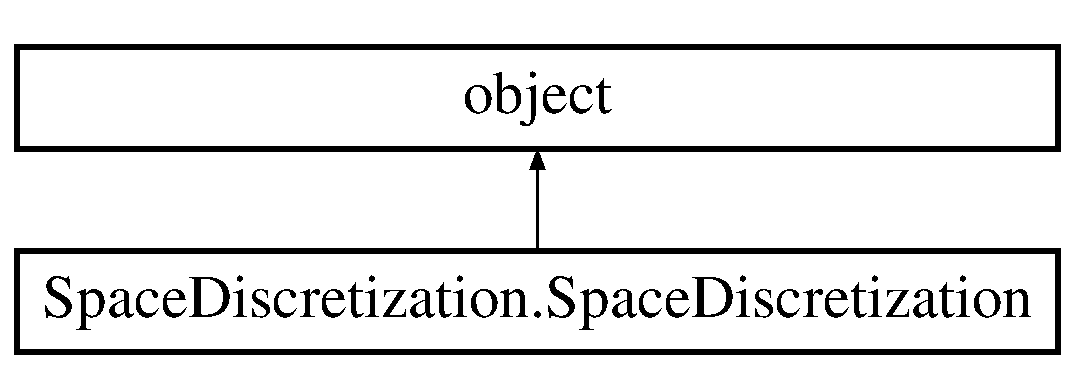
\includegraphics[height=2.000000cm]{class_space_discretization_1_1_space_discretization}
\end{center}
\end{figure}
\subsection*{Public Member Functions}
\begin{DoxyCompactItemize}
\item 
\hypertarget{class_space_discretization_1_1_space_discretization_a94bdc19a1fe63274df51b12fe7246610}{}\label{class_space_discretization_1_1_space_discretization_a94bdc19a1fe63274df51b12fe7246610} 
def {\bfseries \+\_\+\+\_\+init\+\_\+\+\_\+} (self, xmin=0, xmax=100, nx=100, discretization\+\_\+type=\textquotesingle{}linear\textquotesingle{}, x\+\_\+custom=-\/1, angle=0, w=0, soil\+\_\+depth=0, k=1/3600, f=0.\+3, z\+\_\+custom=-\/1)
\item 
\hypertarget{class_space_discretization_1_1_space_discretization_a5ef3a4f5840313a04d3d2436a0183b09}{}\label{class_space_discretization_1_1_space_discretization_a5ef3a4f5840313a04d3d2436a0183b09} 
def {\bfseries space\+\_\+discretization} (self)
\item 
\hypertarget{class_space_discretization_1_1_space_discretization_afd04c500dbe8f21216fd59bff419e5d2}{}\label{class_space_discretization_1_1_space_discretization_afd04c500dbe8f21216fd59bff419e5d2} 
def {\bfseries resample\+\_\+hs1\+D\+\_\+spatial\+\_\+variables} (self)
\item 
\hypertarget{class_space_discretization_1_1_space_discretization_a0ebc4de16ce20df8aecc95011db8b3da}{}\label{class_space_discretization_1_1_space_discretization_a0ebc4de16ce20df8aecc95011db8b3da} 
def {\bfseries get\+\_\+angle\+\_\+node} (self)
\item 
\hypertarget{class_space_discretization_1_1_space_discretization_a54803482692a79a53166ab249e7423d4}{}\label{class_space_discretization_1_1_space_discretization_a54803482692a79a53166ab249e7423d4} 
def {\bfseries get\+\_\+w\+\_\+node} (self)
\item 
\hypertarget{class_space_discretization_1_1_space_discretization_a35f1ce4aa220ecfa59ca1b00154a7b1c}{}\label{class_space_discretization_1_1_space_discretization_a35f1ce4aa220ecfa59ca1b00154a7b1c} 
def {\bfseries get\+\_\+soil\+\_\+depth\+\_\+node} (self)
\item 
\hypertarget{class_space_discretization_1_1_space_discretization_a5451b90853a74e7cd628f3ff1e6c447d}{}\label{class_space_discretization_1_1_space_discretization_a5451b90853a74e7cd628f3ff1e6c447d} 
def {\bfseries set\+\_\+matrix\+\_\+properties} (self)
\item 
\hypertarget{class_space_discretization_1_1_space_discretization_ad9030cbe32bfe65a88357d13a5343d45}{}\label{class_space_discretization_1_1_space_discretization_ad9030cbe32bfe65a88357d13a5343d45} 
def {\bfseries compute\+\_\+x\+\_\+node} (self)
\item 
\hypertarget{class_space_discretization_1_1_space_discretization_aa3a377f7760c5db0e355c76bab8604a0}{}\label{class_space_discretization_1_1_space_discretization_aa3a377f7760c5db0e355c76bab8604a0} 
def {\bfseries compute\+\_\+dx\+\_\+edges} (self)
\item 
\hypertarget{class_space_discretization_1_1_space_discretization_a5e8b2ecac016dc566186b6107f0be117}{}\label{class_space_discretization_1_1_space_discretization_a5e8b2ecac016dc566186b6107f0be117} 
def {\bfseries compute\+\_\+dx\+\_\+node} (self)
\item 
\hypertarget{class_space_discretization_1_1_space_discretization_a64f03ff63047b80235e7e9b660261a8a}{}\label{class_space_discretization_1_1_space_discretization_a64f03ff63047b80235e7e9b660261a8a} 
def {\bfseries first\+\_\+derivative\+\_\+upstream} (self)
\item 
\hypertarget{class_space_discretization_1_1_space_discretization_a4f588e12d85d5af2d9b792dda937139d}{}\label{class_space_discretization_1_1_space_discretization_a4f588e12d85d5af2d9b792dda937139d} 
def {\bfseries first\+\_\+derivative\+\_\+downstream} (self)
\item 
\hypertarget{class_space_discretization_1_1_space_discretization_ad6586556ae92f411631faeabe0c302a5}{}\label{class_space_discretization_1_1_space_discretization_ad6586556ae92f411631faeabe0c302a5} 
def {\bfseries first\+\_\+derivative\+\_\+centered} (self)
\item 
\hypertarget{class_space_discretization_1_1_space_discretization_a19ed0024e755471b382ead47d5c1f5e3}{}\label{class_space_discretization_1_1_space_discretization_a19ed0024e755471b382ead47d5c1f5e3} 
def {\bfseries weight\+\_\+matrix} (self)
\item 
\hypertarget{class_space_discretization_1_1_space_discretization_afa2801eb9367c0b4b0524f1a49fa6658}{}\label{class_space_discretization_1_1_space_discretization_afa2801eb9367c0b4b0524f1a49fa6658} 
def {\bfseries weight\+\_\+matrix\+\_\+bis} (self)
\end{DoxyCompactItemize}
\subsection*{Public Attributes}
\begin{DoxyCompactItemize}
\item 
\hypertarget{class_space_discretization_1_1_space_discretization_ae57fc4d7995e1dcea9716c021100e4e2}{}\label{class_space_discretization_1_1_space_discretization_ae57fc4d7995e1dcea9716c021100e4e2} 
{\bfseries xmin}
\item 
\hypertarget{class_space_discretization_1_1_space_discretization_a8157a0f94c041e799d81fdbd8f90e298}{}\label{class_space_discretization_1_1_space_discretization_a8157a0f94c041e799d81fdbd8f90e298} 
{\bfseries xmax}
\item 
\hypertarget{class_space_discretization_1_1_space_discretization_a85dcc8b930ce51a2c058e884de095d81}{}\label{class_space_discretization_1_1_space_discretization_a85dcc8b930ce51a2c058e884de095d81} 
{\bfseries discretization}
\item 
\hypertarget{class_space_discretization_1_1_space_discretization_a5f7a093a0e5e8b8bdfafe4cd184d5b3a}{}\label{class_space_discretization_1_1_space_discretization_a5f7a093a0e5e8b8bdfafe4cd184d5b3a} 
{\bfseries xcustom}
\item 
\hypertarget{class_space_discretization_1_1_space_discretization_a3e3a0e4330c5dc2c568c56ca9cb42b5b}{}\label{class_space_discretization_1_1_space_discretization_a3e3a0e4330c5dc2c568c56ca9cb42b5b} 
{\bfseries x\+\_\+edges}
\item 
\hypertarget{class_space_discretization_1_1_space_discretization_a55ef88e251ed18338eb0e799d12dc069}{}\label{class_space_discretization_1_1_space_discretization_a55ef88e251ed18338eb0e799d12dc069} 
{\bfseries Hs}
\item 
\hypertarget{class_space_discretization_1_1_space_discretization_a56a4faa92123180a77d2a3f48e982340}{}\label{class_space_discretization_1_1_space_discretization_a56a4faa92123180a77d2a3f48e982340} 
{\bfseries x\+\_\+node}
\item 
\hypertarget{class_space_discretization_1_1_space_discretization_ab1b34a2467e9037acf66652f8b3313c4}{}\label{class_space_discretization_1_1_space_discretization_ab1b34a2467e9037acf66652f8b3313c4} 
{\bfseries N\+\_\+edges}
\item 
\hypertarget{class_space_discretization_1_1_space_discretization_a89c51118aa8928702128d579f7fe4ede}{}\label{class_space_discretization_1_1_space_discretization_a89c51118aa8928702128d579f7fe4ede} 
{\bfseries N\+\_\+nodes}
\item 
\hypertarget{class_space_discretization_1_1_space_discretization_a7f3d9aab32c76477ee2c325dd919f95c}{}\label{class_space_discretization_1_1_space_discretization_a7f3d9aab32c76477ee2c325dd919f95c} 
{\bfseries w\+\_\+node}
\item 
\hypertarget{class_space_discretization_1_1_space_discretization_ac2d3fd91c27fe804fa574d5d3b5ae7d4}{}\label{class_space_discretization_1_1_space_discretization_ac2d3fd91c27fe804fa574d5d3b5ae7d4} 
{\bfseries angle\+\_\+node}
\item 
\hypertarget{class_space_discretization_1_1_space_discretization_ac3b08690e821eff62551b3ecfc2a0646}{}\label{class_space_discretization_1_1_space_discretization_ac3b08690e821eff62551b3ecfc2a0646} 
{\bfseries soil\+\_\+depth\+\_\+node}
\item 
\hyperlink{class_space_discretization_1_1_space_discretization_a09c1380b2ad5b4b86e9bb5761a9bfb9f}{a}
\begin{DoxyCompactList}\small\item\em \mbox{[} 0 ... \end{DoxyCompactList}\item 
\hypertarget{class_space_discretization_1_1_space_discretization_ad8a2df2594d488ebffb9138bec64df3a}{}\label{class_space_discretization_1_1_space_discretization_ad8a2df2594d488ebffb9138bec64df3a} 
{\bfseries b}
\item 
\hypertarget{class_space_discretization_1_1_space_discretization_a5a7cda60432e15fa2e5e3d22ffe769ee}{}\label{class_space_discretization_1_1_space_discretization_a5a7cda60432e15fa2e5e3d22ffe769ee} 
{\bfseries omega}
\item 
\hypertarget{class_space_discretization_1_1_space_discretization_aa9d09433b16461cf836288a2ca250418}{}\label{class_space_discretization_1_1_space_discretization_aa9d09433b16461cf836288a2ca250418} 
{\bfseries omega2}
\item 
\hyperlink{class_space_discretization_1_1_space_discretization_a1a9a27f1f3c729cc06b517b806b8549b}{dx\+\_\+edges}
\begin{DoxyCompactList}\small\item\em \mbox{[}-\/1 1 0 0 0 ... \end{DoxyCompactList}\item 
\hypertarget{class_space_discretization_1_1_space_discretization_a86a03f29332a90545e355b1fc4cbf5f8}{}\label{class_space_discretization_1_1_space_discretization_a86a03f29332a90545e355b1fc4cbf5f8} 
{\bfseries dx\+\_\+node}
\item 
\hyperlink{class_space_discretization_1_1_space_discretization_abdcfc72586714aff94e58dfbe1a91f6d}{c}
\begin{DoxyCompactList}\small\item\em \mbox{[} 0 1 0 0 ... \end{DoxyCompactList}\end{DoxyCompactItemize}


\subsection{Detailed Description}
\begin{DoxyVerb}    Class defining the discretization in space of the hillslope (linear, log, etc....)
    It's detirmined using X minimal and maximal values, soil depth, angle and width
    of the hillslope for each mesh

    @param :
      - xmin : minimal coordinate of the hillslope
      - xmax : maximal coordinate of the hillslope
      - nx : number of cells to define (if x_custom == -1)
      - discretization_type : type of discretization used : 'linear', 'logarithmic',
          'square' or 'custom'
      - x_custom : -1 or vector of coordinates if discretization_type == 'custom'
      - angle : float or vector of values corresponding to the slope
      - w : float or vector of values corresponding to the width
      - soil_depth : float or vector of values corresponding to the thickness of the layer
      - k : hydraulic conductivity
      - f: porosity
      - z_custom : -1 or a vector altitude of each cell (used to compute the slope
           if x_custom is a vector)

    @attributes:
      - xmin : minimal coordinate of the hillslope
      - xmax : maximal coordinate of the hillslope
      - discretization : type of discretization used
      - xcustom : -1 or vector of coordinates if discretization_type == 'custom'
      - b : computation matrix
      - a : computation matrix
      - omega : computation matrix
      - omega2 : computation matrix
      - x_node : coordinates of cells nodes
      - angle_node : slope of cells on nodes
      - w_node : width of cells on nodes
      - N_node : number of cells
      - soil_depth_node : layer thickness on nodes
      - dx_node : distance between two successive nodes
      - x_edges : coordinates of cells edges
      - N_edges : number of cells edges
      - dx_edges : distance between two successive edges
      - Hs : class Hs1D
\end{DoxyVerb}
 

\subsection{Member Data Documentation}
\hypertarget{class_space_discretization_1_1_space_discretization_a09c1380b2ad5b4b86e9bb5761a9bfb9f}{}\label{class_space_discretization_1_1_space_discretization_a09c1380b2ad5b4b86e9bb5761a9bfb9f} 
\index{Space\+Discretization\+::\+Space\+Discretization@{Space\+Discretization\+::\+Space\+Discretization}!a@{a}}
\index{a@{a}!Space\+Discretization\+::\+Space\+Discretization@{Space\+Discretization\+::\+Space\+Discretization}}
\subsubsection{\texorpdfstring{a}{a}}
{\footnotesize\ttfamily Space\+Discretization.\+Space\+Discretization.\+a}



\mbox{[} 0 ... 

0 0 ... 0 \mbox{]} \mbox{[}-\/1 1 0 0 ... 0 \mbox{]} B = \mbox{[} 0 -\/ 1 1 0 ... 0 \mbox{]} \mbox{[}... ... ... ... ... ...\mbox{]} \mbox{[} 0 ... ... 0 -\/ 1 1 \mbox{]} \mbox{[} 0 ... 0 0 ... 0 \mbox{]} size B (Nx + 1) x(\+Nx) \hypertarget{class_space_discretization_1_1_space_discretization_abdcfc72586714aff94e58dfbe1a91f6d}{}\label{class_space_discretization_1_1_space_discretization_abdcfc72586714aff94e58dfbe1a91f6d} 
\index{Space\+Discretization\+::\+Space\+Discretization@{Space\+Discretization\+::\+Space\+Discretization}!c@{c}}
\index{c@{c}!Space\+Discretization\+::\+Space\+Discretization@{Space\+Discretization\+::\+Space\+Discretization}}
\subsubsection{\texorpdfstring{c}{c}}
{\footnotesize\ttfamily Space\+Discretization.\+Space\+Discretization.\+c}



\mbox{[} 0 1 0 0 ... 

0\mbox{]} C = \mbox{[} -\/1 0 1 0 ... 0\mbox{]} \mbox{[} ... ... ... 1\mbox{]} \mbox{[} 0 ... ... 0 -\/ 1 0\mbox{]} \hypertarget{class_space_discretization_1_1_space_discretization_a1a9a27f1f3c729cc06b517b806b8549b}{}\label{class_space_discretization_1_1_space_discretization_a1a9a27f1f3c729cc06b517b806b8549b} 
\index{Space\+Discretization\+::\+Space\+Discretization@{Space\+Discretization\+::\+Space\+Discretization}!dx\+\_\+edges@{dx\+\_\+edges}}
\index{dx\+\_\+edges@{dx\+\_\+edges}!Space\+Discretization\+::\+Space\+Discretization@{Space\+Discretization\+::\+Space\+Discretization}}
\subsubsection{\texorpdfstring{dx\+\_\+edges}{dx\_edges}}
{\footnotesize\ttfamily Space\+Discretization.\+Space\+Discretization.\+dx\+\_\+edges}



\mbox{[}-\/1 1 0 0 0 ... 

0 \mbox{]} A = \mbox{[} 0 -\/ 1 1 0 0 ... 0 \mbox{]} \mbox{[}... ... ... ... ... ... ...\mbox{]} \mbox{[} 0 ... ... ... 0 -\/ 1 1 \mbox{]} size A = (Nx) x(Nx + 1) 

The documentation for this class was generated from the following file\+:\begin{DoxyCompactItemize}
\item 
process/simulation/Space\+Discretization.\+py\end{DoxyCompactItemize}

%--- End generated contents ---

% Index
\backmatter
\newpage
\phantomsection
\clearemptydoublepage
\addcontentsline{toc}{chapter}{Index}
\printindex

\end{document}
